% -*- TeX-master: "../fat_manual.tex" -*-

\section{RHUL West Bond Bonding Machine}

\begin{enumerate}
\item  \cmd{Turn  on   the  machine  by  flicking   the  switch  near
    \quote{Did you book your session?}}
\item \cmd{Turn  on pump  under machine}  - \red{it  will not  make a
    sound as it only needs to pressurize the tank occasionally. It is
    a passive element};
\item \cmd{\red{Turn the valve horizontal}} to connect the pump tank;
\item \cmd{Secure sample};
\item Typical  settings for Aluminum or  Gold.  \red{\textbf{Aluminum
      is easier to bond with}}:
  \begin{itemize}
  \item Buffer 1 or 3;
  \item Power 311;
  \item Time 33ms.
  \end{itemize}
\item Touch = one peek = begin bond,\hspace{1cm} Touch again = double
  peek = terminate bond;
\item \red{\textbf{Move only up or down!}};
\item If the  wire pops out or  breaks \red{do not pull  the wire out
    from  the tube  - its  impossible  to put  back in}.   \cmd{Flick
    \quote{Open}\ira put the wire from  the back though the very end
    of   the  tip}   (where   the  hole   is)   \ira  \cmd{Flick   to
    \quote{feed}};
\item Once done \cmd{pump off  \ira valve to vertical closed position
    \ira power off.}
\end{enumerate}

If not bonding try to:
\begin{itemize}
\item Rewire;
\item Remove needle with Alan key \red{making sure not to drop it!}
\item Clean the  needle with acetone, IPA and ultrasound  \ira dry to
  clean the very tip;
\item Replace needle, so top bit sticks out a little bit.
\end{itemize}

\red{Bong  ground  planes  a  much  as  possible,  and  6  bonds  for
  transmission lines as seen below}

 \begin{center}
   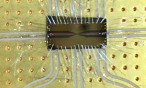
\includegraphics[height=3cm]{bonding}
 \end{center}

 \newpage
